\subsection{Линейные формы (функционалы). Сопряженное (дуальное) пространство. Контрвариантный и ковариантный законы преобразования координат.}

\deff{def:} $V$ - линейное пространство над полем $K$, $f:V \rightarrow  K$ - линейная:
$$\forall \lambda \in K: \forall  v_1,v_2 \in V: f(v_1+ \lambda v_2) = f(v_1)+ \lambda f(v_2)$$
Такое $f$ называется \deff{линейной формой} или \deff{функционалом}.

\textbf{Примеры:}

\begin{enumerate}
    \item $\overline{b} = const: \forall \overline{a}: \in V_3: f(\overline{a}) = (\overline{a},\overline{b})$ - очевидно линейная форма
    \item $A_{n\times n}: f(A) = tr (A)$ - очевидно линейная.
    \item $p \in P$, $\, t_0 \in k \text{ фикс.} \, f(p)= \frac{p^{(m)}t_0}{m!}$ - линейная форма.
    \item $f\in \mathbf{C}(\mathbf{R})$ - бесконечномерное линейное пр-во. $\delta(f)=f(0)$ --- дельта-функция Дирака.
\end{enumerate}

$f_1, f_2$ - линейные формы. Введем операции:
\begin{enumerate}
    \item \textbf{Сложение:} $(f_1+f_2)(v) = f_1(v) + f_2(v)$
    \item \textbf{Умножение на скаляр:}  $(\lambda f_1) (v) = \lambda f_1(v)$
\end{enumerate}
Очевидно существует ноль и противоположные. Откуда выполнены аксиомы 1-8, откуда линейное пространство. 

$V^* = \{f: V \rightarrow K \text{ - линейная форма}\}$ - называется \deff{сопряженное} пр-во к $V$ или \deff{дуальное}.

Возьмем $V$, зафиксируем  $e_1,\ldots,e_n$ - базис.

$\forall X \in V: X\in \sum\limits_{i=1}^nx_i e_i = x^ie_i$ - вспоминаем правило Энштейна из первого семестра. Тогда:
$$X \xleftrightarrow{e}\begin{pmatrix}
    x^1 \\
    x^2 \\
    \vdots \\
    x^n
\end{pmatrix} =x$$ 
$f(X) = f(x^ie_i) = x^if(e_i) = x^ia_i$, где $f(e_i) = a_i \in K$. $f(X) = a_1x^1+a_2x^2 + \ldots + a_n x^n$.

$f \leftrightarrow a= (a_1,\ldots, a_n)$ строка. %Цитата: то есть теперь  у нас функции описываются строками, расписать более подробно(это я себе)
$V^* = (K^n)^T$. 

Откуда $\dim V^*  = n$. 
Это взаимооднозначное соответствие, оно очевидно линейно, откуда это изоморфизм.

То есть теперь на самом деле функции описываются строками --- значениями на базисных векторах.



\textbf{Пример:} 

 Возьмем и посмотрим на скалярное произведение в
$V_3, \, \bar{b}= const$. $\forall X \in V_3, \, f(\bar{X})=(\bar{X}, \bar{b})$.

$f(\bar{i})=(\bar{i}, \bar{b}) = b_1$, $f(\bar{j})=(\bar{j}, \bar{b}) = b_2$, $f(\bar{k})=(\bar{k}, \bar{b}) = b_3$

$\bar{X}=a_1\bar{i}+a_2\bar{j}+a_3\bar{k}$

$f(\bar{X})=a_1b_1+a_2b_2+a_3b_3, $ у нас строка $f \leftrightarrow (b_1,b_2,b_3)$

\deff{def:} $V$, $e = (e_1,\ldots, e_n)$ базис.

$\forall x \in V: w^i(x) = x^i$ --- $i$-ая координата вектора $x$ относительно базиса $e$.  

$w^i$ называется \deff{координатной функцией}.

Не трудно заметить, что $w^i$ - линейная форма $\in V^{*}$.

\thmm{Теорема 1: (о базисе $V^*$)}

Доказать $w^1,\ldots,w^n$ - базис $V^*$.

\textbf{Доказательство:}

Докажем порождаемость: 

$\forall f \in V^*: \forall x \in V: f(x) = x^i a_i = w^i(x)a_i$, где $a_i \in K$ --- порождаемое

Докажем линейную независимость, показав единственность разложения нуля:

$\zero = \alpha_i w^i $, где $\alpha_i \in K$. Посмотрим на $\forall x \in V: \, \alpha_iw^i(x)=\zero$.

Пусть $x = e_j$ для $j = 1,\ldots, n$. Как мы знаем, для $i\neq j: w^i(e_j) = 0$. Тогда $\alpha_iw^i(e_j)=\alpha_j =0$,
$\forall j \Rightarrow $ лин. независим.

\hfill Q.E.D.

\textbf{Следствие:} $w^i$ координатные формы относительно базиса $e$
$\Rightarrow \forall f \in V^*: f = a_iw^i$, т.е $a=(a_1,\ldots,a_n)$  координаты $f$ в базисе $w = (w^1,\ldots, w^n)$ пространства $V^*$.

\textbf{Доказательство:}

$$\forall f \in V^*, \forall x \in V: f(x) = x^ia_i = w^i(x)a_i = (a_iw^i)(x) \Leftrightarrow f = a_iw^i.$$

\hfill Q.E.D.


\deff{def:} $w^1,\ldots, w^n$ называется \deff{сопряженным} (дуальным) к базису $e$ пространства $V$.

Очевидно $w^j(e_i) = \delta^i_j$.

\thmm{Теорема 2:}

$\forall$ базиса $w'^1,\ldots, w'^n$ пространства $V^*$.

$\exists$ базис $e'_1, \ldots, e'_n$ пространства $V$ такой, что $w'$ базис, сопряженный к $e'$. То есть $w'^{i} $ координаты формы относительно $e'$.

\textbf{Доказательство:}


Пусть $e_1,\dots ,e_n \text{ базис } V$. Тогда, как мы говорили ранее:
$ w^1,\dots,w^n $ координатные функции относительно $e$, базис $V^*$ сопряженный к $e$.

Возьмем $w'$. Так как он базис и $w$ базис, то: $$ w' =wT_{w \rightarrow w'}$$
$(T_{w \to w'})^T=S=(S^i_j)_{n\times n}$. Заметим, что $S$ невырожденная, т.к. $T$ матрица перехода. Строки матрицы $S$ --- это координаты элементов нового базиса $w'$ в старом базисе ($w$).
$$(w'^1,\ldots,w'^n)=(w^1,\ldots,w^n)T_{w \to w'}$$
Давайте все транспонируем:
$$\begin{pmatrix}
    w'^1 \\
    \vdots \\
    {w'}^n
\end{pmatrix} = (T_{w \to w'})^T \begin{pmatrix}
    w^1 \\
    \vdots \\
    {w}^n
\end{pmatrix}= S \begin{pmatrix}
    w^1 \\
    \vdots \\
    {w}^n
\end{pmatrix}$$
Пусть $S^{-1}=:T=(t^i_j)_{n \times n}$ --- невырожденная, то если думать о ней как о $T_{e \to e'}$, получим, что $ e' = eT$ базис в пр-ве $V$.

Осталось показать, что $w'$ будет сопряженным к $e'$, т.е. показать ${w'}^{ i}(x)={x'}^i, \, x = {x'}^i {e'}_i$, для всех $ x \in V$. Тк $w'^i$ - линейная форма, то:
$${w'}^i({x'}^i{e'}_j)= {x'}^j {w'}^i(e'_j)$$
Теперь, давайте заметим, что ${w'}^i=S^i_kw^k$, $e'_j = t^m_je_m$. Откуда 
$$ {w'}^i(e'_j)=  S^i_kw^k(t^m_je_m)  = S_k^jt_{j}^m w^k(e_m) = S^i_mt^m_j=(ST)^i_j = $$

% не понял эту строчку, вот есть из записи старых лекций:
% \omega'^i(x) = (S^i_j\omega^j)(x) = S^i_j\omega^j(x) = S^i_jx^j = S^i_jt^j_kx'^k = (ST)^i_kx'^k = \delta^i_kx'^{k} = x'^i
\hfill Q.E.D.

\textbf{Следствие.} $e,e'$ базисы $V$, $w,w'$ сооответственные сопряженные базисы к $e,e'$ в $V^*$.

$T = T_{e\rightarrow e'}, S = T^{-1}$

$ \Rightarrow \forall x \in V: \forall f \in V^*:x' = Sx, a' = aT$, где $a$ - разложение $f$ в базисе.

\textbf{Доказательство:}    

$T=T_{e\rightarrow e'}$ и мы уже знаем, что $x' = T_{e'\rightarrow e}x = Sx$ 

$(T_{w\rightarrow w'})^T = S$. Как мы знаем из матрицы перехода:
$$a^T = T_{w\rightarrow w'}(a')^T$$ 
Откуда:
$$a = a'(T_{w\rightarrow w'})^T = a'S$$
А уже отсюда получаем, что $a' = aS^{-1} = aT$.

\hfill Q.E.D.

\textbf{Замечание от Славы.} Очень удобно менять базис, когда у нас один из базисов канонический. А также, зная матрицу перехода $T_{w\rightarrow w'}$ мы уже знаем матрицу перехода из $T_{e\rightarrow e'} =((T_{w\rightarrow w'})^T)^{-1} $


Преобразование координат, согласованных по тому же закону, что и базис:
$a' =a T$

Преобразование координат, согласованных по противоположному закону:
$x' = Sx$

\deff{def:} Преобразование координат векторов пространства $V$ происходит по закону, противоположному преобразованию базисов --- называется \deff{контрвариантным}, а координаты векторов пространства $V$ называются \deff{контрвариантыми} (индексы координат пишутся вверху).

\deff{def:} Преобразование координат векторов пространства $V$ происходит по тому же закону, что преобразование базисов в пространстве $V$ (т.е. согласованно) называется \deff{ковариантным} преобразованиям.
Координаты векторов пространства $V^* $ называется \deff{ковариантным} (индексы пишутся внизу).

Позамечаем интересные факты:

$\forall f \in V^* \leftrightarrow (a_1,\ldots, a_n), a_j = f(e_j)$ - каждой функции, как и говорилось ранее, на заданном базисе, я могу сопоставить $a$. Поэтому возьму $n$ функций и векторов, и захочу посчитать значение каждой функции в каждой точке : 

$\forall f^1, \ldots f^n \in V^*: f^j \xleftrightarrow{w} a^j = (a_1^j,\ldots , a_n^j)$

$\forall x_1, \ldots, x_n \in V: x_i \xleftrightarrow{e}x_i = \begin{pmatrix}
    x^1_i \\
    \vdots \\ 
    x^n_i
\end{pmatrix}$

Хочу посчитать вот такую вот страшную матрицу (значение каждой функции в каждой точке):

$(f^j(x_i))_{n\times n} = \begin{pmatrix}
    f^1(x_1) & f^1(x_2) & \dots & f^1(x_n)\\
    f^2(x_1) & f^2(x_2) & \dots & f^2(x_n)\\
    \vdots & \ddots & \ddots & \vdots \\
    f^n(x_1) & f^n(x_2) & \dots & f^n(x_n)\\
\end{pmatrix} = f^j(x_i)= a^j x_i  = $


$=\begin{pmatrix}
    a_1^1 & \ldots & \ldots& a^1_n\\ 
     a_1^2 & \ddots & \ddots& a^2_n\\ 
      \vdots & \ddots & \ddots& \vdots\\ 
      a_1^n & \ldots & \ldots& a^n_n\\ 
\end{pmatrix} \cdot\begin{pmatrix}
    x_1^1 & \ldots & \ldots& x^1_n\\ 
     x_1^2 & \ddots & \ddots& x^2_n\\ 
      \vdots & \ddots & \ddots& \vdots\\ 
      x_1^n & \ldots & \ldots& x^n_n\\ 
\end{pmatrix} = \begin{pmatrix}
    f^1\\
    f^2\\
    \vdots\\
    f^n
\end{pmatrix} \cdot \begin{pmatrix}
    x_1 & x_2 & \ldots & x_n
\end{pmatrix}$ - лаконичная запись!



Интересный факт, который идет из такого произведения:
$$\begin{pmatrix}
    w^1 \\
    w^2 \\
    \vdots \\
    w^n \\
\end{pmatrix} \cdot (e_1e_2 \dots e_n) = E $$

\deff{def:} $V^{**} = (V^*)^*$ \deff{дважды сопряженное} пространство.

$\forall f \in V^*$. Пусть $x \in V$:

$"x"(f) = f(x)$. $"x": V^* \rightarrow K$.

$\forall \lambda \in K: \forall f^1,f^2 \in V^*$

$"x"(\lambda f^1+f^2) = (\lambda f^1 + f^2)(x) = \lambda f^1(x) + f^2(x) = \lambda_1 "x"(f^1) + "x"(f^2)$

$\Rightarrow "x"$ линейное отображение $\Rightarrow"x" \in (V^*)^*$

Дальше у $"x"$ будут упускаться "" :))

\thmm{Теорема 3 (О естественном изоморфизме)}

Естественный - не зависит от введения базиса.

$V \cong V^{**}$

\textbf{Доказательство:}

$\forall x \in V \rightarrow "x"\in V^{**}$. Назовем это отображение $\varphi$.

Покажем, что наше взаимооднозначное сопоставление линейно.

$x_1 + \lambda x_2 \in V: x_1 \rightarrow "x_1"$, $x_2 \rightarrow "x_2"$


$\forall f\in V^*: "x_1+\lambda x_2"(f) = f(x_1+\lambda x_2) = f(x_1) + \lambda f(x_2) = "x_1"(f) + \lambda"x_2"(f) $. Откуда $\varphi$ линейно.

\begin{center}
    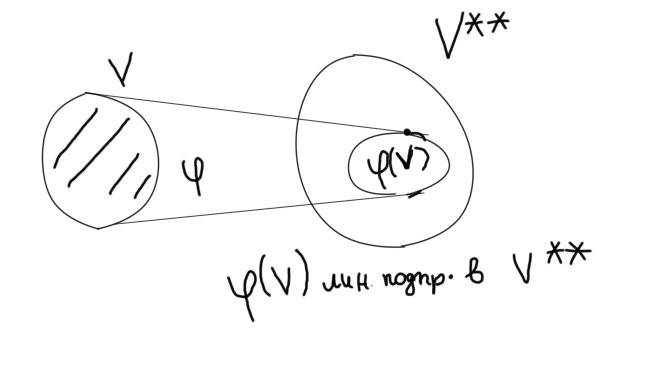
\includegraphics[width =15cm]{assets/8_1-varphi-linear.png}
\end{center}

Покажем, что $\varphi$, это изоморфизм.

Пусть $e_1,\ldots, e_n$ базис $V$. Им соответствуют $ "e_1"$$,\ldots, "e_n"$. Покажем, что это базис в $V^{**}$:

Мы знаем, что $\dim (V^*)^* = \dim V^* = \dim V = n$. Откуда достаточно показать, что $"e_1"$ $,\ldots, "e_n"$ - линейно независимы. Для этого покажем единственность разложения нуля.

$0= \sum\limits_{i=1}^n \alpha_i "e_i"(w_i)=\sum\limits_{i=1}^n\alpha_i w^j(e_j) = \alpha_j \Rightarrow$ линейно независимы, откуда базис.

Откуда отображение $\varphi$ это изоморфизм.

\hfill Q.E.D.

Как мы только что поняли: $x \in V \leftrightarrow "x" \in V^{**}$ - изомофризм. $f\in V^{*}, x \in V$.

$x(f)= f(x) = x^i a_i = w^i(x) a_i = x(w^i)a_i =x^ia_i=x^i f(e_i)=x^ie_i(f)$

$e \text{ и }w$ взаимно сопряж.

$x=x^ie_i, w^i(x)=x^i,$ где $x \in V$

$e_j(f)=f(e_j)=a_j(f \in V^*)$, $e_j \in V^{**}$ - коорд. формы относительно базиса $w^i$.

Я категорически не помню для чего Кучерук это написала, напомните мне пж.





\textbf{Пример:}

$\mathcal{A}$ - о.п.с, $A$ - диагонализируема.

$V = \bigoplus\limits_{\lambda}V_{\lambda} = \span (v_1,\ldots,v_n)$

$w^1,\ldots,w^n$ сопряж. базис к $v$  % дописать

$\Rightarrow \forall x \in V: w^j(x) =x^i: x^iv_j = x$ 

\newpage
\subsection{Два определения тензора. Линейное пространство тензоров. Многомерная матрица тензоров.}

\deff{def:} Есть $V,V^*$ и $p,q \in N$.

\deff{Тензором} типа $(p,q)$ ($p$-раз ковариантным, $q$-раз контрвариантным) называется полилинейная функция $f: V^p\times (V^*)^q \rightarrow K$. $p,q$ называются \deff{валентностями} тензора, $r = (p+q)$ ранг тензора.

Если $r = 0, f = const$. Если тензор $(p,0) $ - \deff{ковариантный} тензор валентности $p$. Если тензор $(0,q)$ - \deff{контрвариантный} тензор валентности $q$. Если $p\neq 0 $ и $q\neq 0$ - тензор смешанного типа.

$\xi_j \in V, \eta^i \in V^*$

$f(\xi_1,\ldots,\xi_p,\eta^1,\ldots, \eta^q)$ - линейно по каждому аргументу (или полилинейная)

Пусть $e = (e_1,\ldots, e_n)$ - базис $V$, $w = (w^1,\ldots, w^n)$ - базис $V^*$. Тогда сделаем похожую вещь, как когда мы считали определитель. По линейности вынесем, то есть:
$$\xi_j = \xi_j^{j_k}e_{j_k};\eta^i = \eta_{i_m}^iw^{i_m}$$
$$f(\xi_1,\ldots,\xi_p,\eta^1,\ldots, \eta^q) = \xi_1^{j_1}\ldots\xi_p^{j_p}\eta_{i_1}^1 \ldots \eta^q_{i_p} \cdot f(e_{j_1},\ldots, e_{j_p},w^{i_1},\ldots, w^{i_q})$$
То есть  на самом деле наша функция задается матрицей значений на базисных векторах. Обозначим $f(e_{j_1},\ldots, e_{j_p},w^{i_1},\ldots, w^{i_q}) = \alpha_{j_1,\ldots,j_p}^{i_1,\ldots,i_q}$

\deff{def:} $M$ - \deff{многомерная матрица} тензора $r = (p+q)$ мерная размерности $n$. 

\textbf{Замечание:} Если говорить программистким языком, то наша матрица это просто:

\begin{lstlisting}[mathescape]
for (i1 = 1 ... n):
    for(i2 = 1 ... n):
        ...
        for(iq = 1 ... n):
            for(j1 = 1 ... n):
                ...
                for(jp = 1 ... n):
                    m[i1][i2]...[iq][j1]...[jp] = f($\text{соответсвенных значений}$)
\end{lstlisting}

\deff{Соглашение о записи элементов многомерной матрицы}

$\alpha^{i_1,\ldots,i_q}_{j_1,\ldots, j_p} \in M_{p+q}$ - многомерная матрица порядка $n$. $i_k \in (1,\ldots,n); j_m \in (1,\ldots, m)$

Мы читаем сначала верхние индексы, потом нижние в записи

\textbf{Пример:}
\begin{enumerate}
    

\item $r =2: (\alpha^i_j), (\alpha^{ij}),(\alpha_{ij})$

$1$-ый индекс номер строки

$2$-ой индекс номер столбца

Например при $n= 3$:

$(a^{i}_j) = \begin{pmatrix}
    \alpha^{1}_1 &\alpha^1_2 & \alpha_3^1\\
    \alpha_1^2 & \alpha_2^2 & \alpha_3^2 \\
    \alpha_1^3 & \alpha_2^3 & \alpha_3^3
\end{pmatrix}$ 
или 
$(a^{ij}) = \begin{pmatrix}
    \alpha^{11} &\alpha^{12} & \alpha^{13}\\
    \alpha^{21} & \alpha^{22} & \alpha^{23} \\
    \alpha^{31} & \alpha^{32} & \alpha^{33}
\end{pmatrix}$ 

\item $r=3: (\alpha^{ijk}), (\alpha^{ij}_k), (\alpha^{i}_{jk}), (\alpha_{ijk}) $

    1-ый индекс всегда строка

    2-ой индекс всегда столбец

    3-ий индекс всегда слой

Например при $n=3$:

$(a^i_{jk}) = \left(
\begin{array}{ccc|ccc|ccc}
    \alpha^1_{11} & \alpha^1_{21} & \alpha^1_{31} & \alpha^1_{12} & \alpha^1_{22} & \alpha^1_{32} & \alpha^1_{13} & \alpha^1_{23} & \alpha^1_{33} \\
    \alpha^2_{11} & \alpha^2_{21} & \alpha^2_{31} & \alpha^2_{12} & \alpha^2_{22} & \alpha^2_{32} & \alpha^2_{13} & \alpha^2_{23} & \alpha^2_{33} \\
    \alpha^3_{11} & \alpha^3_{21} & \alpha^3_{31} & \alpha^3_{12} & \alpha^3_{22} & \alpha^3_{32} & \alpha^3_{13} & \alpha^3_{23} & \alpha^3_{33}
\end{array}
\right)$

\item $r=4: (\alpha^{ijkm}),(\alpha^{ijk}_{m}),(\alpha^{ij}_{km}), (\alpha^{i}_{jkm}), (\alpha_{ijkm})$

1-ый индекс всегда строка

2-ой индекс всегда столбец

3-ий индекс всегда слой

4-ый индекс всегда сечение

Например при $n=2$ мы имеем:

$(a^{ij}_{km}) = \left(
\begin{array}{cc|cc}
  \alpha^{11}_{11} & \alpha^{12}_{11} & \alpha^{11}_{12} & \alpha^{12}_{12} \\
  \alpha^{21}_{11} & \alpha^{22}_{11} & \alpha^{21}_{12} & \alpha^{22}_{12} \\
\hline
  \alpha^{11}_{21} & \alpha^{12}_{21} & \alpha^{11}_{22} & \alpha^{12}_{22} \\
  \alpha^{21}_{21} & \alpha^{22}_{21} & \alpha^{21}_{22} & \alpha^{22}_{22} \\
\end{array}
\right)$


\item $r=1: (\alpha^i), (a_i)$ 

При первой записи мы считаем, что она в столбик, а при второй считаем, что она строчка.

\end{enumerate}


\textbf{Пример:} 

$f:V_3\times V_3 \rightarrow \mathbb{R}$

$\forall \overline{a}, \overline{b}: f(\overline{a},\overline{b}) = |\overline{a}||\overline{b}|\cos \varphi$

$f\in T(2,0)$. Зафиксируем базис $e_1,e_2,e_3$:

$f(a^ie_i,b^jr_j) = a^ib^j f(e_i,e_j)$

Пусть $e_1,e_2,e_3$ вектора, между которыми $2$ угла по $60$ градусов и $1$ $120$  и $|e_i|=i$.

Тогда $(a_{ij})= \begin{pmatrix}
    1 & 1 & \cfrac{3}{2} \\
    1 & 4& 3 \\
    \cfrac{3}{2} & 3 & 9
\end{pmatrix}$


\textbf{Вернемся в реальность}.

Пускай $f \in T(p,q) \xleftrightarrow{e,w} \left(\alpha^{i_1,\ldots,i_q}_{j_1,\ldots,j_p}\right)$, где $e$ - базис, $w$ - дуально сопряженный

$f: V^p \times (V^*)^q\rightarrow K$

Возьмем $e' = (e_1',\ldots,e_n' )$ и дуальный к нему $w'=(w'_1,\ldots, w'_m)$

$T = T_{(e\rightarrow e')}, S = T^{-1} = (T_{w\to w'}^T)$

Замечу, что $\xi =\xi^i e_i: \xi = T \xi' \leftrightarrow \xi^i = t_k^i\xi'^k$
и $\eta = \eta_j w^j; \eta = \eta'S \leftrightarrow \eta_j = s_{j}^k \eta'_k $

Возьму $\xi_1,\ldots,\xi_p \in V$ и $\eta^1,\ldots, \eta^q\in V^*$:
$$f(\xi_1,\ldots,\xi_p,\eta^1,\ldots,\eta^q)=\alpha^{i_1,\ldots,i_q}_{j_1,\ldots, j_p}\xi_1^{j_1}\ldots \xi_{p}^{j_p} \eta_{i_1}^1 \ldots \eta_{iq}^q =\alpha^{i_1,\ldots,i_q}_{j_1,\ldots, j_p} \cdot t_{k_1}^{j_1}\xi_1'^{k_1}\ldots t_{k_p}^{{j_p}}\xi'^{k_p}_p \cdot s_{i_1}^{m_1}\eta'^1_{m_1}\ldots s_{i_q}^{m_q}\eta'^1_{m_q}$$
$$= \alpha^{i_1,\ldots i_q}_{j_1,\ldots, j_p} \cdot t_{k_1}^{j}\ldots t_{k_p}^{j_p}\cdot s_{i_1}^{m_1}\ldots s_{i_q}^{m_q}\cdot \xi_1'^{k_1}\ldots \xi_{p}'^{k_p} \cdot \eta'^{1}_{m_1}\ldots \eta'^{q_1}_{m_q}$$
Откуда подставив новые базисные вектора в эту формулу:
$$\alpha_{k_1,\ldots,k_p}'^{\,m_1,\ldots, m_q} = \alpha_{j_1,\ldots,j_p}^{i_1,\ldots, i_q}t_{k_1}^{j_1}\ldots t_{k_p}^{j_p}\ldots s_{i_1}^{m_1}\ldots s_{i_q}^{m_q}$$
$j_1,\ldots, j_p$ ковариантные индексы матрицы, $i_1,\ldots, i_q$ контрвариантные, откуда название тензора $f\in T(p,q)$ $p$-раз ковариантный, $q$ раз контрвариантный.

\textbf{Замечание:} это формула перехода (смены базиса), потом будет очень много везде использоваться.


\deff{2-ое определение тензора:} $\alpha$ --- $r = p+q$ мерная матрица $n$ - геометрический объект над пространством $V$ $(\dim V =n)$, такой, что при смене базиса пространства $V$ элементы матрицы пересчитываются по формуле:
$$\alpha_{k_1,\ldots,k_p}'^{m_1,\ldots, m_q} = \alpha_{j_1,\ldots,j_p}^{i_1,\ldots, i_q}t_{k_1}^{j_1}\ldots t_{k_p}^{j_p} s_{i_1}^{m_1}\ldots s_{i_q}^{m_q}$$(геометрический объект - независимый от выбора базиса, но согласованный с заменой базиса, т.е. после замены базиса остается тем же объектом с теми же свойствами)

Если матрицы одного порядка, то мы умеем складывать их и умножать на скаляр, есть нулевая и противоположная, откуда это линейное пространство.  

Осталось показать, что эти операции не ломают второе определение (формулу перехода):
$$(\alpha + \lambda \beta)_{k_1,\ldots,k_p}'^{\,m_1,\ldots,m_q} = \alpha_{k_1,\ldots,k_p}'^{\, m_1,\ldots, m_q} + \lambda \beta_{k_1,\ldots,k_p}'^{\, m_1,\ldots, m_q} = \alpha_{j_1,\ldots,j_p}^{i_1,\ldots,i_q} \cdot t_{k_1}^{j_1} \ldots t_{k_p}^{j_p}\cdot s_{i_1}^{m_1}\ldots s_{i_q}^{m_q} + \lambda\beta_{j_1,\ldots,j_p}^{i_1,\ldots,i_q} \cdot t_{k_1}^{j_1} \ldots t_{k_p}^{j_p}\cdot s_{i_1}^{m_1}\ldots s_{i_q}^{m_q} $$
$$= (\alpha_{j_1,\ldots, j_p}^{i_1,\ldots,i_q} + \lambda \beta_{j_1,\ldots, j_p}^{i_1,\ldots,i_q})t_{k_1}^{j_1}\ldots s_{i_q}^{m_q}$$
Откуда корректно.

\textbf{Замечание:} в дальнейшем мы будем называть формулу перехода - свойством линейного пространства.

То есть теперь наше линейное пространство сохраняет заданное свойство.


Заметим, что мы получили равносильность первого и второго определения.


\subsection{Произведение тензоров. Базис пространства тензоров. Свертка тензоров.}

\deff{def:} $\alpha \in T(p_1,q_1),\beta \in T(p_2,q_2)$. Тогда \deff{произведением} тензоров называется тензор $\gamma \in T(p_1+p_2,q_1+g_2):$ 
$$\gamma^{i_1,\ldots i_{q_1},m_1,\ldots,m_{q_2}}_{j_1,\ldots,j_{p_1},k_1,\ldots, k_{p_2}}:= \alpha^{i_1\ldots i_q}_{j_1,\ldots,j_p} \beta^{m_1,\ldots,m_{q_2}}_{k_1,\ldots, k_{p+2}}$$
Проверим корректность, то есть то что выполняется свойство тензора:
$$\gamma_{\widetilde{j_1},\ldots,\widetilde{j}_{p_1}, \widetilde{k}_1,\ldots, \widetilde{k}_{p_2}}'^{\, \widetilde{i_1},\ldots,\widetilde{i}_{q_1}, \widetilde{m}_1,\ldots, \widetilde{m}_{q_2}} = \alpha_{\widetilde{j_1},\ldots,\widetilde{j}_{p_1}}'^{\, \widetilde{i_1},\ldots,\widetilde{i}_{q_1}} \cdot \beta_{ \widetilde{k}_1,\ldots, \widetilde{k}_{p_2}}'^{\,\widetilde{m}_1,\ldots, \widetilde{m}_{q_2}} = $$
$$= \alpha_{j_1,\ldots j_{p_1}}^{i_1,\ldots, i_{q_1}} t_{\widetilde{j}_1}^{j_1}\ldots t_{\widetilde{j}_{p_1}}^{j_{p_1}} s_{i_1}^{\widetilde{i}_1}\ldots s_{i_{q_1}}^{\widetilde{i}_{q_1}}\cdot \beta_{k_1,\ldots k_{p_2}}^{m_1,\ldots, m_{q_2}} t_{\widetilde{k}_1}^{k_1}\ldots t_{\widetilde{k}_{p_2}}^{k_{p_2}} s_{m_1}^{\widetilde{m}_1}\ldots s_{m_{q_2}}^{\widetilde{m}_{q_2}} = $$
$$=\gamma_{j_1,\ldots,j_{p_1},k_1,\ldots , k_{p_2}}^{i_1,\ldots, i_{q_1}, m_1,\ldots,m_{q_2}}\cdot t_{\widetilde{j}_1}^{j_1}\ldots t_{\widetilde{j}_{p_1}}^{j_{p_1}} s_{i_1}^{\widetilde{i}_1}\ldots s_{i_{q_1}}^{\widetilde{i}_{q_1}}\cdot t_{\widetilde{k}_1}^{k_1}\ldots t_{\widetilde{k}_{p_2}}^{k_{p_2}} s_{m_1}^{\widetilde{m}_1}\ldots s_{m_{q_2}}^{\widetilde{m}_{q_2}}$$
Откуда получаем, что верно, это тензор!!! \sout{я устал это писать}

Обозначается $\gamma = \alpha \otimes \beta$.

Произведение ассоциативно, дистрибутивно, не коммутативно



\textbf{Пример:}

Пусть $\alpha \in T(1,0), \beta \in T(0,1)$. Тогда $\gamma = \alpha \otimes \beta  \in T(1,1)$.

$\alpha = (\alpha_1,\alpha_2,\alpha_3); \beta =(\beta_1,\beta_2,\beta_3)^T$. Тогда
$$\gamma^i_j =\alpha^i\beta_j \leftrightarrow \gamma = \begin{pmatrix}
    \alpha^1\beta_1 &\alpha^1\beta_2 & \alpha^1 \beta_3 \\
    \alpha^2\beta_1 &\alpha^2\beta_2 & \alpha^2 \beta_3 \\
     \alpha^3\beta_1 &\alpha^3\beta_2 & \alpha^3 \beta_3 \\
\end{pmatrix}$$



Возьмем $\alpha \in T(p_1,q_1) \leftrightarrow f: V^{p_1}\times(V^{q_1})^* \rightarrow K$. 

Возьмем $\beta \in T(p_2,q_2) \leftrightarrow g: V^{p_2}\times(V^{q_2})^* \rightarrow K$.

$\xi_1,\ldots, \xi_{p_1} \in V;\eta^1,\ldots, \eta^{q_1}\in V^*;\zeta_1,\ldots, \zeta_{p_2}\in V; \theta^1,\ldots, \theta^{q_2}\in V^*$

$\gamma = a \otimes \beta \in T(p_1+p_2, q_1+q_1)\leftrightarrow t: V^{p_1+p_2}\times (V^*)^{q_1+q_2}\rightarrow K$
$$t(\xi_1,\ldots,\xi_{p_1},\zeta_1,\ldots,\zeta_{p_2}, \eta^1,\ldots, \eta^{q_1},\theta^1,\ldots, \theta^{q_2}) =$$$$= \gamma_{j_1,\ldots,j_{p_1},k_1,\ldots,k_{p_2}}^{i_1,\ldots,i_{q_1},m_1,\ldots,m_{q_2}} \xi_1^{j_1}\ldots \xi_{p_1}^{j_{p_1}}\cdot \zeta_1^{k_1}\ldots \zeta_{p_2}^{k_{p_2}} \cdot \eta^1_{i_1}\ldots \eta_{i_{q_1}}^{q_1} \cdot \theta_{m_1}^1 \ldots \theta^{q_2}_{m_{q_2}} = $$
$$=f(\xi_1,\ldots, \xi_{p_1},\eta^1,\ldots, \eta^{q_1})\cdot g(\zeta_1,\ldots \zeta_{p_2}, \theta^1,\ldots \theta^{q_2}) $$
Вывели формулу, по которой мы можем легко находить значения функций. Воспользуемся нашей формулойd и выведем еще одну:

$f^1,\ldots , f^p \in V^* = T(1,0)$ --- $f^j:V\rightarrow K$  - линейная форма

$g_1,\ldots,g_q\in V^{**} = T(0,1)$ --- $g_i:V^*\rightarrow K$

$\gamma = f^1\otimes \ldots \otimes f^p \otimes g_1 \otimes \ldots \otimes g_q \leftrightarrow a^1_{j1}\ldots a^{p}_{j_p}b_1^{i_1}\ldots b_q^{i_q}= \gamma^{i_1,\ldots, i_q}_{j_1,\ldots, j_p}$, $\gamma \in T(p,q)$.

Воспользуемся только что доказанной формулой и получим:
$$\gamma(\xi_1,\ldots \xi_p, \eta^1,\ldots, \eta^q)= f^1(\xi_1)\ldots f^q(\xi_q)\cdot g_1(\eta^1)\ldots g_q(\eta^q)$$
Продолжим играться с этой формулой:

Пусть $f^j = w^j$, а $g_i = e_i$ (сопряженные базисы), и подставим это в нашу формулу:

$w^{j_1} \otimes \ldots \otimes w^{j_p} \otimes e_{i_1} \otimes \ldots \otimes  e_{i_q}\in T(p,q) $

Как мы вывели ранее:
$$w^{j_1}\otimes \ldots \otimes w^{j_p} \otimes e_{i_1}\otimes \ldots \otimes e_{i_q} (\xi_1,\ldots , \xi_p, \eta^1,\ldots,\eta^q) = w^{j_1}(\xi_1)\ldots w^{j_p}(\xi_q)\cdot e_{i_1}(\eta^1)\ldots e_{i_q}(\eta^q) = $$
$$=\xi_1^{j_1}\xi_2^{j_2}\ldots \xi_p^{j_p} \cdot \eta_{i_1}^1 \ldots \eta_{i_q}^q $$
Получили вот такую относительно простую формулу для базисных векторов


\thmm{Теорема (о базисе пространства тензоров типа ($p$, $q$))}

Набор тензоров $w^{j_1}\otimes \ldots \otimes w^{j_p} \otimes e_{i_1}\otimes \ldots \otimes e_{i_q}$, где $j_k \in (1,\ldots,n),i_m\in(1,\ldots,n)$ --- базис пространства $T(p,q)$.

\textbf{Доказательство:}

\begin{enumerate}
    \item Докажем, что порождающее. Пусть $f\in T(p,q): \forall \xi_1,\ldots \xi_p \in V, \forall \eta^1,\ldots \eta^q\in V^*:$

    Давайте найдем значение функции в этой точке:
    $$f(\xi_1,\ldots, \xi_p,\eta^1,\ldots, \eta^q) = \alpha_{j_1,\ldots,j_p}^{i_1,\ldots,i_q}\xi_1^{j_1}\ldots \xi_{p}^{j_p}\cdot \eta_{i_1}^1 \ldots \eta_{i_q}^q = $$
    Выразим координаты через базис и дуальный к нему:
    $$=\alpha_{j_1,\ldots,j_p}^{i_1,\ldots,i_q} w^{j_1}(\xi_1)\ldots w^{j_p}(\xi_p) e_{i_1}(\eta^1)\ldots e_{i_q}(\eta^q) = \alpha_{j_1,\ldots,j_p}^{i_1,\ldots,i_q} w^{j_1}\otimes \ldots \otimes p_{i_q}(\xi_1,\ldots, \eta^q)$$
    Что мы получили? Разложение в нашем базисе с коэффициентами: $\alpha_{j_1,\ldots,j_p}^{i_1,\ldots,i_q} $

    Откуда порождаемо.
    \item Докажем, что линейно независимо. Для этого, как обычно, покажем единственность разложения нуля:
    $$\gamma = \alpha_{j_1,\ldots, j_p}^{i_1,\ldots,i_q}w^{j_1}\otimes\ldots\otimes w^{j_p}\otimes e_{i_1}\otimes \ldots \otimes e_{i_q}=\zero$$
    Давайте подставим какие-то базисные векторы:
    $$\gamma(e_{\widetilde{j}_1},\ldots, e_{\widetilde{j}_p}, w^{\widetilde{i}_1},\ldots, w^{\widetilde{i}_q}) = $$
    $$\alpha_{j_1,\ldots,j_p}^{i_1,\ldots,i_q}w^{j_1}(e_{\widetilde{j}_1})\ldots w^{j_p}(e_{\widetilde{j}_p}) \cdot e_{i_1}(w^{\widetilde{i}_1})\ldots e_{i_q}(w^{\widetilde{i}_q})$$
    Заметим, что каждая из $w^{j_k}(e_{\widetilde{j}_k}) = \delta_{\widetilde{j}_k}^{j_k}$ и $e_{i_k}(w^{\widetilde{i}_k}) = \delta^{\widetilde{i}_k}_{i_k}$, поэтому получим, что:
    $$ = \alpha_{\widetilde{j}_1,\ldots,\widetilde{j}_p}^{\widetilde{i}_1,\ldots, \widetilde{i}_q}$$
    Но с другой стороны это ноль (тк мы смотрим на разложение тензора, выдающего всегда ноль (нуля)). Тогда получаем, что все $\alpha = 0$, откуда единственно
\end{enumerate}

\hfill Q.E.D.

\textbf{Следствие:} элементы матрицы тензора это его координаты в базисе пространства $T(p,q): w^{j_1}\otimes \ldots\otimes w^{j_p}\otimes e_{i_1}\otimes \ldots \otimes e_{i_q}$

С одной стороны элементы матрицы - значения на базисном наборе, а с другой стороны коэффициент при базисном элементе.


\textbf{Замечание.} Канонический базис состоит из тензоров, в матрицах которых есть ровно одна единица, а все остальные значения нули.

\deff{def:} Пусть $\alpha \in T(p,q): p,q \geq 1$, тогда тензор $\beta$ называется \deff{сверткой} тензора $\alpha$, если
$$\beta^{i_1,\ldots, \widehat{i}_k,\ldots,i_q}_{j_1,\ldots,\widehat{j}_m,\ldots,j_p} = \alpha_{j_1,\ldots,j_{m-1}, \ae,j_{m+1},\ldots,j_p}^{i_1,\ldots,i_{k-1},\ae, i_{k+1},\ldots,i_q}$$
Причем $\widehat{i}_k$ - нет индекса на этой позиции.

\textbf{Замечание:} Этого не говорили на лекции, но $k,m$ фиксированы. Отсюда я бы хотел написать похожее определение, которое может быть более понятным:
$$\beta_{j_1,\ldots,j_{m-1},j_{m+1},\ldots,j_p}^{i_1,\ldots,i_{k-1},i_{k+1},\ldots,i_q} = \alpha_{j_1,\ldots,j_{m-1}, \ae,j_{m+1},\ldots,j_p}^{i_1,\ldots,i_{k-1},\ae, i_{k+1},\ldots,i_q}$$
(Причем тут скрыта сумма в правой части)

Получили, что $\beta \in T(p-1,q-1)$, но нам осталось проверить свойство:
$$\beta_{\widetilde{j_1},\ldots,\hat{\widetilde{j}}_m,\ldots,\widetilde{j}_p}'^{\widetilde{i}_1,\ldots,\hat{\widetilde{i}}_k,\ldots, \widetilde{i}_q} =\alpha_{\widetilde{j_1},\ldots,\ae,\ldots,\widetilde{j}_p}'^{\widetilde{i}_1,\ldots,\ae,\ldots, \widetilde{i}_q} = $$
$$= \alpha_{j_1,\ldots,j_m,\ldots,j_p}^{i_1,\ldots,i_k,\ldots,i_q} \cdot t_{\widetilde{j}_1}^{j_1}\ldots t^{j_m}_{\ae}\ldots t^{j_p}_{\widetilde{j}_p}\cdot s_{i_1}^{i_1}\ldots s^{\ae}_{i_k}\ldots s_{i_q}^{\widetilde{i}_q} = $$
Что у нас происходит с $\ae$? Мы умножаем $j_m$ строчку $T$ на $i_k$ строчку $S$, откуда $t^{j_m}_{\ae} \cdot s_{i_k}^{\ae} = (TS)_{i_k}^{j_m} =\delta_{i_k}^{j_m}$. Тогда в нашей сумме сохранится только суммы, когда $i_k = j_m = \widetilde{\ae} $:
$$=\alpha_{j_1,\ldots,\widetilde{\ae},\ldots,j_p}^{i_1,\ldots, \widetilde{\ae},\ldots, i_q}t_{\widetilde{j}_1}^{j_1}\ldots \widehat{t^{j_m}_{\ae}}\ldots t^{j_p}_{\widetilde{j}_p}\cdot s_{i_1}^{i_1}\ldots \widehat{s^{\ae}_{i_k}}\ldots s_{i_q}^{\widetilde{i}_q}$$
(переменные с крышками как бы пропали)

Откуда получили то, что нужно.

\textbf{Замечание:} Свертка может происходить по нескольким парам символов.

\textbf{Замечание:} Если в результате свертки получалась константа, то такая свертка называется \deff{полной}.


\newpage
\subsection{Транспонирование тензора. Симметричные, кососимметричные тензоры.}

Пускай $\alpha \in T(2,0), \alpha = (\alpha_{ij})$, мы умеем ее транспонировать --- $\alpha^T =(a_{ij})^T =\beta = (\beta_{ij}),$ причем $\beta_{ij} = \alpha_{ji}$. Это называется транспонированием 2-мерной матрицы.
Казалось бы, можно транспонировать многомерную матрицу, но нет так нельзя

Для тензоров транспонирование происходит только по одному типу индексов \uline{либо по нижним, либо по верхним}.

Пускай $\beta = \alpha^T$. $\beta_{j_1j_2} = \alpha_{j_2j_1}$. На самом деле случилась перестановка. Теперь для тензора произвольного типа

\deff{def:} $\alpha \in T(p,q), p\geq 2$. Пусть $\sigma$ это перестановка из $p$ чисел $(1,2,3,\ldots, p)$. $\sigma = (\sigma_1,\ldots,\sigma_p)$

$\beta = \sigma(\alpha)$. $\beta$ получен \deff{транспонированием} (перестановкой $\sigma$) по нижним индексам из тензора $\alpha$ по перестановке $\sigma$, если
$$\beta_{j_1\ldots j_p}^{i_1,\ldots i_q} = \alpha_{j_{\sigma_1 \ldots j_{\sigma_p}}}^{i_1,\ldots i_q}$$
\textbf{Замечание.} Аналогично определяется транспонирование по верхним индексам.

\textbf{Замечание.} При транспонировании по нижним индексам верхние индексы никак не задействованы.

\textbf{Замечание.} В дальнейшем мы будем рассматривать транспонирования по нижним индексам. Все, что будет доказано для транспонированя и по нижним индексам будет выполнено и для транспонирования по верхним индексам.

Как и было раньше нам надо проверить корректность определение тензора(то самое свойство).

$\forall \sigma$ = конечное число транспозиций двух элементов(доказывали в прошлом семестре). То есть достаточно проверить корректность определения для транспонирования при котором переставляются только 2 индекса.


$\beta_{j_1, \ldots* \ldots  \Delta \ldots j_p}^{i_1\ldots i_q}= \alpha_{j_1, \ldots \Delta\ldots  * \ldots j_p}^{i_1\ldots i_q}$, где $*$ и $\Delta$ - наша перестановка.
$$\beta_{m_1.\ldots m_{*}\dots m_{\Delta}\ldots m_p}'^{\, k_1 \ldots k_q} = \alpha_{m_1.\ldots m_{\Delta}\dots m_{*}\ldots m_p}'^{\, k_1 \ldots k_q}  = \alpha^{i_1 \ldots i_1}_{j_1\ldots \Delta \ldots * \ldots  j_p}t_{m_1}^{j_1} \ldots t_{m_\Delta}^{j_\Delta}\ldots t_{m_*}^{j_*} \ldots t_{m_p}^{j_p}s_{i_1}^{k_1}\ldots s_{i_q}^{k_q}$$
Заметим, что $\alpha_{j_1\ldots \Delta\ldots *\ldots j_p} = \beta_{j_1\ldots * \ldots \Delta \ldots j_p}^{i_1 \ldots i_q}$, переставим множители $t_{m_\Delta}^{j_\Delta}, t_{m_*}^{j_*}$ и получим наше определение.

\textbf{Теперь посмотрим на это с функциональной стороны:}

$\alpha \in T(p,q) \leftrightarrow f: V^p \times (V^*)^q \rightarrow K$, $\beta = \sigma(\alpha) \leftrightarrow g: V^p\times (V^*)^q\rightarrow K$

$\forall \xi_1,\xi_2,\ldots, \xi_p \in V;\forall \eta^1,\ldots,\eta^q \in V^*:$
$$g(\xi_1, \ldots, \xi_p, \eta^1,\ldots, \eta^q) = \beta_{j_1\ldots j_p}^{i_1.\ldots i_q} \xi_1^{j_1}\ldots \xi_{p}^{j_p}\eta_{i_1}^1 \ldots \eta_{i_q}^q = \alpha_{j_{\sigma_1}\ldots j_{\sigma_p}}^{i_1\ldots i_q} \xi_1^{j_1}\ldots \xi^{j_p}_p \eta_{i_1}^1 \ldots \eta_{i_q}^q $$
Немного переставим внутри и получим:
$$=\alpha_{j_{\sigma_1}\ldots j_{\sigma_p}}^{i_1\ldots i_q} \xi_{\sigma_1}^{j_{\sigma_1}}\ldots \xi^{j_{\sigma_p}}_{\sigma_p} \eta_{i_1}^1 \ldots \eta_{i_q}^q = f(\xi_{\sigma_1},\ldots \xi_{\sigma_p}, \eta^1,\ldots, \eta^q)$$
То есть:
$$g = \sigma(f) \leftrightarrow g(\xi_1,\ldots, \xi_p, \eta^1, \ldots, \eta^q) = f(\xi_{\sigma_1},\ldots \xi_{\sigma_p}, \eta^1,\ldots, \eta^q)$$

\textbf{Пример:}

Пусть $\alpha \in T(3,0)$, $\alpha = f^1 \otimes f^2 \otimes f^3, f^j \in V^* = T(1,0)$, $\sigma = (312), \beta = \sigma(\alpha)$.

$\forall \xi_1,\xi_2,\xi_3 \in V$

$\beta(\xi_1,\xi_2,\xi_3) = \alpha(\xi_3,\xi_1,\xi_2) = f^1\otimes f^2 \otimes f^3 (\xi_3,\xi_1,\xi_2) = f^1(\xi_3)\cdot f^2(\xi_1)\cdot f^3(\xi_2)$

И из этого примера следует формула:

Если $\alpha \in T(p,q): \alpha = f^1 \otimes \ldots \otimes f^p \otimes \gamma $, $\beta = \sigma(\alpha)$,$p\geq 2$, $\gamma \in T(0,q)$

$\beta = f^{\sigma_1^{-1}}\otimes \ldots \otimes f^{\sigma_p^{-1}} \otimes \gamma = \sigma^{-1}(f^1\otimes \ldots \otimes f^p) \otimes \gamma$

На практике транспонирование многомерной матрицы тензора осуществляется:

\deff{МЕТОДОМ ТРАНСПОНИРОВАНИЯ СЛОЯМИ:}

Для этого разобьем нашу $\sigma$ на транспозиции и будем транспонировать по ним по очереди:

Для этого фиксируется набор верхних индексов,  и набор нижних индексов, за исключением двух нижних. Таким образом из многомерной матрицы тензора извлекается двумерная матрица, которая называется \deff{слой}.
$$\alpha^{i_1\ldots i_q}_{j_1 \ldots * \ldots \Delta \ldots j_p}$$ 
Здесь я фиксирую все $i$-шки, а $j$ все фиксированнны кроме $*$  и $\Delta$. Получили двумерную матрицу порядка $n$ - \deff{слой}. 
$$(\alpha_{j_1\ldots * \ldots \Delta \ldots j_p}^{i_1 \ldots i_q})^T = \overline{\alpha}$$
(просто обычная транспозицая квадратной двумерной матрицы).

И после транспонирования слой $\overline{\alpha}$ размещается обратно в исходную матрицу на те же позиции. Таким образом, в тензоре будут произведена перестановка (транспозиция) двух индексов. Назовем такую операцию $\tau$.

Тогда наша последовательность действий выглядит так: 
$$\sigma \xrightarrow{\tau_1}\overline{\sigma}\xrightarrow{\tau_2}\ldots \xrightarrow{} (1,2,\ldots n)$$
\textbf{Пример:}

$n = 4, \alpha \in T(3,0), \sigma = (3 12)\rightarrow \overline{\sigma} =  (132) \rightarrow \overline{\overline{\sigma }} = (123)$

1) Проведем первую операцию. Так как у нас зафиксирована 3-я координата, то на самом деле нам надо лишь транспонировать 3 матрицы слоев. На рисунке снизу изображены все 4-и слоя и матрицы $A_1,A_2,A_3,A_4$. Поэтому для операции транспонирования я должен взять каждую из матриц $A_i$ и транспонировать ее
\begin{center}
         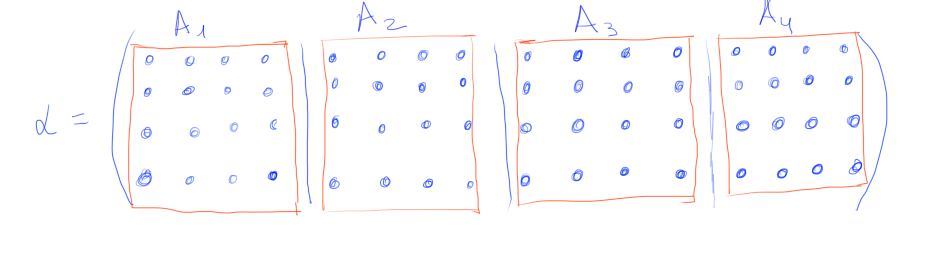
\includegraphics[width = 18cm]{assets/8_4-sample-1.png}
 \end{center}
2) Проведем вторую операцию. В этот раз у нас зафиксирована 1-ая координата(строка). Зафиксируем $i=1$ и выпишем соответствующий ей слой:
\begin{center}
         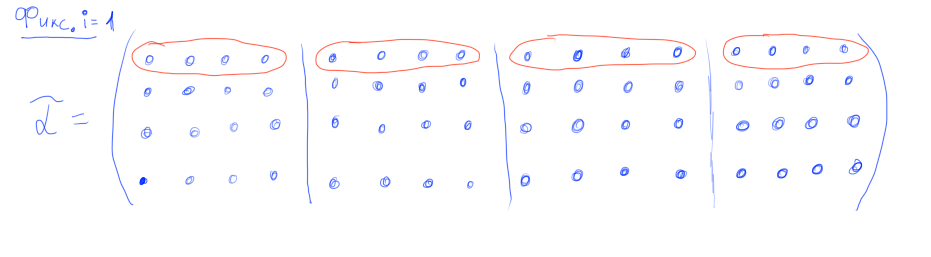
\includegraphics[width = 18cm]{assets/8_4-sample-2.png}
         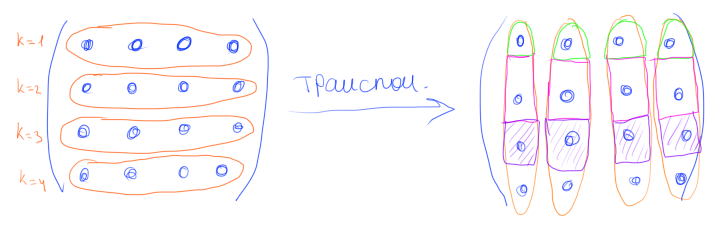
\includegraphics[width = 12cm]{assets/8_4-sample-3.png}
 \end{center}
А теперь возвращаем наш слой обратно. На рисунке показано, как мы это делаем:
 \begin{center}
         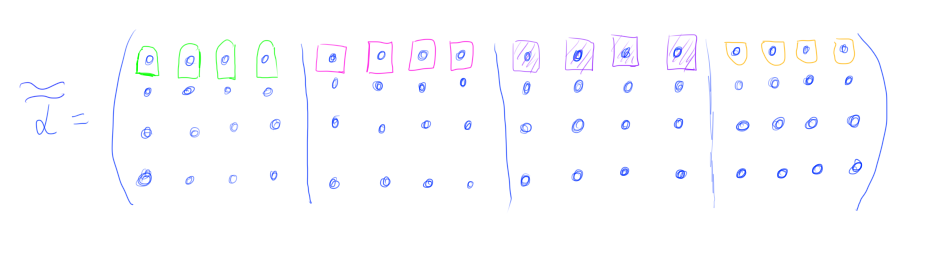
\includegraphics[width = 18cm]{assets/8_4-sample-4.png}
 \end{center}
Проделываем то же самое с остальными 3-емя слоями и получаем протранспонированную матрицу тензора.

\textbf{Замечание:} Если в матрице тензора много нулей, то проще пересчитать элементы по формуле.

\textbf{Замечание:} $\beta =\sigma(\alpha), \sigma = (kij)$. $\alpha_{ikj} = \beta_{kij}$ --- неверно!!! Это ошибка!!!

Операция транспонирования - \uline{линейная операция}, очевидно из определения.

$\sigma = \tau_k \cdot \ldots \tau_1$ произведение перестановок ассоциативно и не коммутативно, откуда операция транспозиции тензора аналогично ассоциативна и не коммутативна.

\deff{def:} $\alpha \in T(p,q)$ называется \deff{симметричным} тензором по нижним индексам, если $\forall \sigma$ перестановки $\sigma(\alpha) = \alpha$

\deff{def:} $\alpha \in T(p,q)$ называется \deff{кососимметричным} тензором по нижним индексам, если $\forall \sigma: \sigma(\alpha) = (-1)^{\varepsilon(\sigma)
}\alpha$, где $\varepsilon$ знак перестановки. (смотрите конспект первого семестра, раздел 6)

Поговорим, про равносильные определения:

$\alpha$ симметричный $\Leftrightarrow \sigma: \alpha_{j_1,\ldots, j_p}^{i_1,\ldots, i_q} = \alpha_{j_{\sigma_1}\ldots j_{\sigma_p}}^{i_1 \ldots i_q} \Leftrightarrow \forall (k,m): \alpha_{\ldots j_k \ldots j_m \ldots}^{i_1,\ldots, i_q} = \alpha_{\ldots j_m \ldots j_k \ldots}^{i_1 \ldots i_q}$

$\alpha$ кососимметричный $\Leftrightarrow \sigma: \alpha_{j_1,\ldots, j_p}^{i_1,\ldots, i_q} = (-1)^{\varepsilon(\sigma)}\alpha_{j_{\sigma_1}\ldots j_{\sigma_p}}^{i_1 \ldots i_q} \Leftrightarrow \forall (k,m): \alpha_{\ldots j_k \ldots j_m \ldots}^{i_1,\ldots, i_q} = -\alpha_{\ldots j_m \ldots j_k \ldots}^{i_1 \ldots i_q}$

Теперь про функциональные:

$\alpha$ - симметричный $\Leftrightarrow \forall \sigma: \forall \xi_1,\ldots , \xi_p \in V; \forall \eta^1,\ldots, \eta^q \in V^*: $
$$\alpha(\xi_1,\ldots, \xi_p,\eta^1,\ldots, \eta^q) = \alpha (\xi_{\sigma_1},\ldots \xi_{\sigma_p
}, \eta^1, \ldots, \eta^q) \Leftrightarrow$$
$$\Leftrightarrow \forall (k,m): \alpha(\ldots, \xi_m, \ldots,\xi_k,\ldots) = \alpha (\ldots, \xi_k,\ldots, \xi_m,\ldots)$$
$\alpha$ - кососимметричный $\Leftrightarrow \forall \sigma: \forall \xi_1,\ldots , \xi_p \in V; \forall \eta^1,\ldots, \eta^q \in V^*: $
$$\alpha(\xi_1,\ldots, \xi_p,\eta^1,\ldots, \eta^q) =(-1)^{\varepsilon(\sigma)} \alpha (\xi_{\sigma_1},\ldots \xi_{\sigma_p
}, \eta^1, \ldots, \eta^q) \Leftrightarrow$$
$$\Leftrightarrow \forall (k,m): \alpha(\ldots, \xi_m, \ldots,\xi_k,\ldots) = -\alpha (\ldots, \xi_k,\ldots, \xi_m,\ldots)$$
\deff{Утверждение.} $\alpha $ кососимметричный $\Leftrightarrow\forall (k,m):\forall \xi: \alpha(\ldots, \xi, \ldots \xi, \ldots ) = 0$

\textbf{Замечание:} $\alpha \in T(p,q)$ --- кососимметричная. Тогда
\begin{enumerate}
    \item Если $p>n \Rightarrow \alpha \equiv \zero$, тк обязательно в наборе $j_1,\ldots, j_p$ будут одни индексы, а из этого следует, что все компоненты будут нулями
    \item Если $p=n \Rightarrow$ ненулевые элементы матрицы $\alpha$ будут только те, у которых набор нижних индексов $j_1,\ldots j_n$ = перестановка от $1$ до $n$. Все остальные будут нулями , тк совпадают индексы:
    $$\alpha_{j_1\ldots j_p}^{i_1\ldots i_q} = (-1)^{\varepsilon(\sigma)}\alpha_{1\ldots n}^{i_1* \ldots i_q}$$
\end{enumerate}

\textbf{Примеры:}

\begin{enumerate}
    \item $V_3$, $\alpha(\overline{a}, \overline{b}) = (\overline{a}, \overline{b})\in T(2,0)$ --- скалярное произведение --- симметрично.
     \item $V_3$, $\alpha(\overline{a}, \overline{b}, \overline{c}) = \overline{a} \overline{b}\overline{c}\in T(3,0)$ --- смешанное произведение --- кососимметрично.
     \item $n =3, \alpha \in T(3,0)$, $\alpha$ - симметрично $\alpha = (\alpha_{ijk})$. Тогда $\alpha_{123}=\alpha_{132}=\alpha_{213}= \alpha_{231} = \alpha_{312} = \alpha_{321}$, $\alpha_{112} = \alpha_{121}  =\alpha_{211}$, $\ldots$. См рисунок

     \begin{center}
         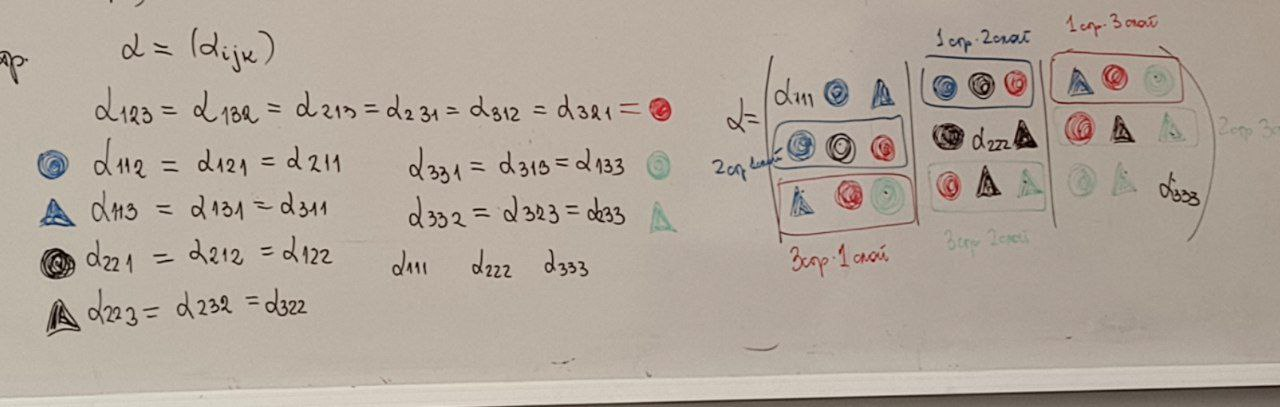
\includegraphics[width = 18cm]{assets/8_4-table.jpg}
     \end{center}
     \sout{он перерисуется, когда у славы руки дойдут}
\end{enumerate}

\pagebreak
\subsection{Операции симметрирования и альтернировании тензора.}

кососимметричный = антисимметричный = альтернированный.

\deff{def:} $\alpha \in T(p,q), p \geq 2$. $\Sim \alpha = \cfrac{1}{p!}\sum\limits_{\sigma \in S_p}\sigma(\alpha)$, где $S_p$ - множество всех перестановок $(1,\ldots, p)$. Такая операция называется \deff{симметрированием} тензора по нижним индексам.

\deff{def:} $\Alt \alpha = \cfrac{1}{p!}\sum\limits_{\sigma \in S_p}(-1)^{\varepsilon(\sigma)}\sigma(\alpha)$ - операция \deff{альтернирования}  тензора по нижним индексам.

\textbf{Замечание:} по верхним аналогичным.

Позамечаем некоторые интересные факты 
\begin{enumerate}
    \item $\Sim \alpha \in T(p,q), \Alt \alpha \in T(p,q) $ 
    \item $\Sim, \Alt$ --- линейные операции, так как $\sigma$ - линейные операторы.
    \item если $\alpha$ симметричный $\Rightarrow \Sim \alpha = \alpha$
    \item  если $\alpha$ кососимметричный $\Rightarrow \Alt \alpha = \alpha$
    \item $\Sim$ и $\Alt$ можно проводить не по всему набору (нижних) индексов. В этом случае, тот набор по которому происходит симметрирование (альтернирование) заключается в круглые (квадратные) скобки. Индексы, не участвующие в операндах выделяются вертикальными чертами. При этом квадратные и круглые скобки должны быть только одни.

\end{enumerate}

\thmm{Теорема.}

$\alpha \in T(p,q), p \geq 2.$ 

$\forall \sigma: \Sim \sigma(\alpha) = \sigma(\Sim \alpha) = \Sim \alpha, \Alt(\sigma(\alpha)) = \sigma(\Alt\alpha) = (-1)^{\varepsilon(\sigma)}\Alt \alpha$

\textbf{Доказательство:}

Будем доказывать для $\Alt$ для ($\Sim$ упр).
$$\Alt (\sigma(\alpha))=\cfrac{1}{p!}\sum\limits_{\tau\in S_p}(-1)^{\varepsilon(\tau)}\tau(\sigma(\alpha))$$
Пусть $r \sigma = \rho$. Заметим, что $\rho$ пробегает все $P$. Тогда заменим и получим:
$$=  \cfrac{(-1)^{\varepsilon(\sigma)}}{p!}\sum\limits_{\rho \in S_\rho} (-1)^{\varepsilon(\rho)}\rho(\alpha)$$
Теперь вторая часть:
$$\sigma(\Alt \alpha) = \sigma\left(\cfrac{1}{p}\sum_{\tau\in S_P}(-1)^{\varepsilon}\tau(\alpha)\right)$$
Как мы знаем транспонирование это линейная операция. Сделаем замену на $\rho$, как в прошлой части и получим:
$$= \cfrac{1}{p!}\sum\limits_{\tau \in S_p}(-1)^{\varepsilon(\tau)}\sigma(\tau(\alpha)) = \cfrac{(-1)^{\varepsilon(\sigma)}}{p!}\sum\limits_{\rho \in S_p}(-1)^{\varepsilon(\tau)} \rho(\alpha)$$
Получили то, что хотели.

\hfill Q.E.D.

\textbf{Следствие 1.} $\forall \alpha \in T(p,q)$, $\Alt \alpha$ - кососимметричный тензор, $\Sim \alpha$ - симметричный тензор. Очевидно по определению.

\textbf{Следствие 2.} $\alpha$ кососимметричный $\Leftrightarrow$ $\Alt \alpha= \alpha$ и $\alpha$ симметричный $\Leftrightarrow \Sim \alpha = \alpha$

\textbf{Доказательство:}

В правую сторону очевидно по определению. Докажем в левую сторону.

Пусть $\alpha = \Alt \alpha$. Тогда $\sigma(\Alt \alpha) = \sigma(\alpha) = (-1)^{\varepsilon(\sigma)}\Alt \alpha = (-1)^{\varepsilon(\sigma)}\alpha$. Откуда $\sigma(\alpha) = (-1)^{\varepsilon(\sigma)} \alpha$. Откуда кососимметрично по определению.

\hfill Q.E.D.

\textbf{Следствие 3.} $\Alt(\Alt \alpha) = \Alt \alpha$, $\Sim(\Sim \alpha) = \Sim \alpha$, $\Alt(\Sim \alpha) = \zero$, $\Sim(\Alt \alpha) = \Sim \alpha$

Очевидно по определению.

\textbf{Замечание.} Теорема и следствия верны для неполного набора индексов.

\textbf{Замечание.} $T(p,q)^{\text{кососим}}$ и  $T(p,q)^{\text{сим}}$ - линейные пространства в $T(p,q)$.

\textbf{Замечание.}$T(p,q)^{\text{кососим}} \oplus T(p,q)^{\text{сим}} = T(p,q)$

\pagebreak

\subsection{p-формы. Внешнее произведение $p$ форм.}

\deff{def:} $f \in T(p,0)$ --- ковариантный тензор валентности $p$ --- \deff{полилинейная форма}.

$f \in T(p,0)$ и \deff{полилинейная антисимметричная} форма = ковар. тензор валентности $p$ и кососимметричный. В таком случае $f$ называется \deff{$p$-формой}, или \deff{внешней формой}, или внешней формой порядка $p$. 

$\Lambda^pV^* = \{f \in T(p,0): \Alt f = f\}$ --- линейное подпространство тензоров --- \deff{линейное пространство} $p$-форм.

$p = 1: \Lambda^1 V^* \equiv V^*$.

\deff{def:} $g\in T(0,q)$ --- \deff{контрвариантный тензор} валентности $q$ или \deff{поливектор}.

$g \in T(0,q)$ --- \deff{антисимметричный поливектор} --- \deff{q-вектор}

$V^qV = \{g\in T(0,q): \Alt g =g\}$ --- \deff{линейное пространство} $q$-векторов.

\textbf{Замечание:} все, что мы выведем для $p$-форм, будет верно и для $q$-форм

\deff{def:} $f^1 \in \Lambda^{p_1}V^*,f^2\in \Lambda^{p_2}V^*$ $p_1$ и $p_2$ формы. Введем новую операцию, такую:
$$f^1 \wedge f^2 = \cfrac{(p_1+p_2)!}{p_1!p_2!}\Alt (f^1\otimes f^2)$$
Такая операция называется \deff{внешним произведением} $p$-форм.

\textbf{Свойства внешнего произведение:}

\begin{enumerate}
    \item $f^1\wedge f^2 = (-1)^{p_1 \cdot p_2} \cdot  f^2 \wedge f^1$
    
    \textbf{Доказательство:}
    $$f^1 \wedge f^2 = \cfrac{(p_1 + p_2)!}{p_1!p_2!} (\Alt f^1 \otimes f^2)$$
    Заметим, что тогда должно быть выполнено:
    $$\Alt (f^1 \otimes f^2)  = (-1)^{p_1\cdot p_2} \Alt(f^2\otimes f^1)$$
    Введем больше формальности в доказательства. Разложим $f^1,f^2$ по базису пространства тензоров. Получим:
    $$f^1 \leftrightarrow (a_{i_1,\ldots i_{p_1}}), f^2 \leftrightarrow (b_{j_1,\ldots, j_{p_2} }) $$
    Тогда давайте выпишем:
    $$f^1 \otimes f^2 \leftrightarrow \gamma_{i_1\ldots i_{p_1}j_1\ldots j_[p_2]} = \alpha_{i_1\ldots i_{p_1} } \beta_{j_1\ldots j_{p_2}}$$
    $$f^2\otimes f^1 \leftrightarrow \theta_{j_1\ldots j_{p_2} i_1\ldots i_{p_1}}  = \beta_{j_1\ldots, j_{p_2}}\alpha_{i_1\ldots i_{p_1}}$$
    Тогда
    $$\Alt (\gamma) = \cfrac{1}{(p_1 + p_2)!} \sum\limits_{\sigma \in S_{p_1+p_2}} \sigma(\gamma)(-1)^{\varepsilon(\sigma)} \quad \Alt(\theta) = \cfrac{1}{(p_1+p_2)!} \sum_{\tau \in S_{p_1+p_2}}\tau(\theta)(-1)^{\varepsilon(\tau)}$$
    Не трудно присмотреться, что в альтернировании второго, мы дополнительно  
     перестановку  из $(i_1,\ldots,i_{p_1},j_1,\ldots, j_{p_2})$ в $(j_1,\ldots, j_{p_2},i_{1},\ldots i_{p_1})$, обозначим ее $ab$ (Заметим, что мы тратим  $p_1\cdot p_2$ транспозиций). То есть на самом деле я применяю к исходному $\alpha$ перестановку, а это значит, что 
    $$\Alt \gamma = \Alt(ab(\theta))=(-1)^{\varepsilon(ab)}\Alt \theta=(-1)^{p_1p_2}\Alt \theta$$

    \hfill Q.E.D.

    В частности, $f^1\in V^*,f^2\in V^*$, то $f^1 \wedge f^2 = -f^2 \wedge f^1$. Так же $f \wedge f = \zero$. 

    Отсюда выводится свойство, что $w^i \wedge w^j = - w^j \wedge w^i$ и $w^i \wedge w^i = \zero$. 

    \item $(f^1+f^2)\wedge f^3 = f^1\wedge f^3 + f^2 \wedge f^3$ и $f^1 \wedge (f^2 + f^3) = f^1 \wedge f^2 + f^1 \wedge f^3$
    \item $\forall \lambda \in K: (\lambda f^1)\wedge f^2 = \lambda(f^1 \wedge f^2) = f^1 \wedge (\lambda f^2)$
    \item $\zero_{\Lambda^{p_1}V^*} \wedge f^2 = f^1 \wedge \zero_{\Lambda^{p_2}V^*}=\zero_{\Lambda^{p_1+p_2}V^*}$
    \item $(f^1 \wedge f^2 ) \wedge f^3 = f^1 \wedge (f^2 \wedge f^3) = f^1 \wedge f^2 \wedge f^3$

    \textbf{Доказательство:}

    Распишем первое:
    $$(f^1 \wedge f^2)\wedge f^3 = \left(\cfrac{(p_1+p_2)!}{p_1! p_2!}\Alt (f^1 \otimes f^2)\right)\wedge f^3 =$$  $$=\cfrac{(p_1 + p_2 + p_3)!}{(p_1+p_2)!(p_3)!} \Alt\left(\left(\cfrac{(p_1+p_2)!}{p_1! p_2} \Alt (f^1 \otimes f^2)\right)\otimes f^3 \right) = \cfrac{(p_1+p_2+p_3)!}{p_1!p_2!p_3!} \Alt \left( \Alt(f^1 \otimes f^2) \otimes f^3 \right)$$
    Распишем второе:
    $$(f^1 \wedge f^2)\wedge f^3 = \cfrac{(p_1+p_2+p_3)!}{p_1!p_2!p_3!} \Alt \left( f^1 \otimes \Alt(f^2 \otimes f^3) \right)$$
    Нам надо лишь доказать, что $\Alt(\Alt(f^1 \otimes f^2)\otimes f^3) = \Alt (f^1 \otimes \Alt (f^2 \otimes f^3))$

    Ну, давайте докажем:
    $$\Alt(\Alt(f^1 \otimes f^2)\otimes f^3) = \Alt \left(\cfrac{1}{(p_1+p_2)!} \sum\limits_{\sigma \in S_{p_1+p_2}}\left((-1)^{\varepsilon(\sigma)}\sigma(f^1\otimes f^2)\otimes f^3\right)\right) $$
    $$f^1 \otimes f^2 \leftrightarrow \alpha_{i_1\ldots i_{p_1}}\beta_{j_1\ldots j_{p_2}} \quad f^3 \leftrightarrow \gamma_{\theta_1\ldots \theta_{p_3}}$$
    
    Заметим, что $\sigma $ это перестановка, которая переставляет $p_1 + p_2$ индексов.

    Возьму $\tau$ такую перестановку, что она переставляет $(p_1+p_2+p_3)$ индексов $i_1,,\ldots, i_{p_1},j_1,\ldots, j_{p_2},\theta_1,\ldots,\theta_{p_3}$, но при этом последние $p$ индексов будут стоять на месте(Расширим нашу перестановку $\sigma$).
    $$= \cfrac{1}{(p_1+p_2)!}\Alt\left(\sum_{\sigma \in S_{p_1+p_2}}(-1)^{\varepsilon(\tau)}\tau(f^1 \otimes f^2 \otimes f^3)\right) = \cfrac{1}{(p_1+p_2)!}\sum\limits_{\sigma} (-1)^{\varepsilon(\tau)}\Alt(\tau(f^1 \otimes f^2 \otimes f^3)) =$$$$= \cfrac{1}{(p_1+p_2)!}\Alt (f^1 \otimes f^2 \otimes f^3)\sum\limits_{\sigma \in S_{p_1+p_2}}1 = \Alt (f^1 \otimes f^2 \otimes f^3)$$
    Аналогичным образом раскрываем и получаем, для другой то же самое. Откуда они равны.


    \hfill Q.E.D

    \textbf{Следствие:} $f^1 \wedge f^2 \wedge f^3 = \cfrac{(p_1 + p_2 + p_3)!}{p_1!p_2!p_3!}\Alt (f^1 \otimes f^2 \otimes f^3)$

    \textbf{Следствие:} По индукции верно $f^1 \wedge \ldots \wedge f^n = \cfrac{(p_1 +\ldots +  p_n)}{p_1!\ldots p_n!} \Alt (f^1 \otimes \ldots \otimes f^n)$

    \textbf{Следствие:} $\forall j = 1 \ldots p: f^j\in V^* = \Lambda^1 V^*$
    $$f^1\wedge \ldots \wedge f^p = p!\cdot \Alt(f^1 \otimes \ldots \otimes f^n)$$
    Это следует из нашего свойства и поэтому у нас именно такое обозначение $p$-форм (у нас как бы значок $\wedge$)

    \item $\forall j=1\ldots p : f^j \in V^*= \Lambda^1V^*$.
    
    Тогда $$\sigma(f^1 \wedge f^2 \wedge \ldots\wedge  f^p) = (-1)^{\varepsilon(\sigma)}f^1\wedge \ldots \wedge f^p = \sigma^{-1}(f^1\wedge \ldots \wedge f^n) = f^{\sigma_1}\wedge \ldots \wedge f^{\sigma_p}$$

    \textbf{Доказательство:}

    Докажем только последний переход, все остальные очевидны из определения:
    $$\sigma^{-1}(f^1 \wedge \ldots \wedge f^p ) = p! \sigma^{-1}\Alt (f^1 \otimes \ldots \otimes f^p ) =p!\Alt (\sigma^{-1}(f^1 \otimes \ldots \otimes f^p)) $$

    \textbf{Следствие:} Если $f^j$--- 1 формы, тогда:
    $$f^1 \wedge \ldots \wedge f^k \wedge \ldots \wedge f^m \wedge \ldots \wedge f^p = -f^1 \wedge \ldots \wedge f^m \wedge \ldots \wedge f^k \wedge \ldots f^P$$
    $$\ldots \wedge f \wedge \ldots \wedge f \wedge \ldots = \zero$$
\end{enumerate}

\thmm{Теорема (о базисе пространства $p$ - форм)}

Пусть $j_1 < \ldots  < j_p$ --- упорядоченный набор $j_l \in (1,\ldots,n)$

$\{w^{j_1}\wedge \ldots \wedge w^{j_p}\}$ совокупность по всем упорядоченным наборам $(j_1,\ldots, j_p)$ --- базис $\Lambda^pV^*$.

\textbf{Доказательство:}

\deff{Докажем порождаемость:}

$\forall f \in \Lambda^p V^*$. $f\in T(p,0)$ и $f = \Alt f$ - кососимметричный. Разложим по координатам тензора
$$f= \alpha_{i_1\ldots i_p} w^{i_1}\otimes \ldots \otimes w^{i_p}$$
С другой стороны $\Alt f = \Alt (\alpha_{i_1\ldots i_p}w^{i_1}\otimes  \ldots \otimes w^{i_p}) = a_{i_1\ldots i_p}\Alt (w^{i_1}\otimes \ldots \otimes w^{i_p})$. Из следствия 2 свойства 5 $\Alt (w^{i_1}\otimes \ldots \otimes w^{i_p}) = \cfrac{1}{p!}w^{i_1}\wedge \ldots \wedge w^{i_p}$. 

Если среди $(i_1\ldots i_p)$ есть одинаковые индексы, то $w^{i_1} \wedge \ldots \wedge w^{i_p} = \zero$. Если все индексы различные, то это просто перестановка $(j_1,\ldots,j_p): j_1<\ldots <j_p$. Тогда заменим на равное:
$$=\sum_{j_1<\ldots<j_p}\cfrac{1}{p!}\sum\limits_{\sigma \in S_p} \alpha_{j_{\sigma_1}\ldots j_{\sigma_p}} w^{j_{\sigma_1}}\wedge \ldots \wedge w^{j_{\sigma_p}} = \sum_{j_1<\ldots<j_p}\cfrac{1}{p!}\sum\limits_{\sigma \in S_p} \alpha_{j_{\sigma_1}\ldots j_{\sigma_p}} (-1)^{\varepsilon(\sigma)}w^{j_1}\wedge \ldots w^{j^p}$$
Вынесем за скобки и получим:
$$=\sum_{j_1<\ldots<j_p}\left(\cfrac{1}{p!}\sum\limits_{\sigma \in S_p}\alpha_{j_{\sigma_1}\ldots j_{\sigma_p}}(-1)^{\varepsilon(\sigma)}\right)w^{j_1}\wedge \ldots \wedge w^{j_p}$$
Откуда порождаемый.

\textbf{Замечание:} коээффицент перед омегами равен $\beta_{j_1\ldots j_p}$ b называется \deff{существенной} координатой $p$-формы $f$.  Она равна $\alpha_{[j_1\ldots j_p]}=\alpha_{j_1\ldots j_p}$. 

\deff{Докажем линейно-независимость:}

Для этого составим комбинацию. 
$$\zero=\sum\limits_{j_1 <\ldots j_p}\beta_{j_1\ldots j_p} w^{j_1}\wedge \ldots \wedge w^{j_P}= 
\sum\limits_{j_1 < \ldots <j_p} \beta_{j_1\ldots j_p}\sum_{\sigma \in S_p} w^{j_{\sigma_1}}\otimes\ldots\otimes w^{j_{\sigma(p)}} \cdot (-1)^{\varepsilon(\sigma)} = $$
$$= \alpha_{i_1\ldots i_p} w^{i_1}\otimes \ldots \otimes w^{i_p}$$
где если хотя бы 2 индекса совпадают,то $\alpha_{i_1\ldots i_p} = 0$. Получили, что базис из тензоров = нулю, откуда и искомые.

\hfill Q.E.D.

\textbf{Следствие 1:} $\dim \Lambda^pV^* = C^p_n = \cfrac{n!}{p!(n-p)!}$

\textbf{Следствие 2:} $\forall f \in \Lambda^p V^*:$
$$f = \sum\limits_{j_1<\ldots <j_p} \beta_{j_1\ldots j_p}w^{j_1}\wedge \ldots \wedge w^{j_p}$$
где $\beta_{j_1\ldots j_p} = \alpha_{j_1\ldots j_p}$--- 
\deff{существенные} координаты.

Существенные координаты принято записывать в строку
(перестановки в лексикографическом порядке)

\textbf{Пример:}

$n=4, p=3: f\in \Lambda^{p}V^* \leftrightarrow \beta = (\beta_{123},\beta_{124},\beta_{134}, \beta_{234})$

\thmm{Теорема 1}

$\forall \xi_1,\ldots, \xi_p \in V:$ $w^{j_1}\wedge \ldots \wedge w^{j_p} (\xi_1,\ldots,\xi_p) = \det(\xi^{j_m}_k)_{p\times p} = \begin{vmatrix}
    \xi_1^{j_1} & \ldots & \xi_p^{j_1}\\
    \vdots & & \vdots \\
    \xi_1^{j_p} & \ldots & \xi_p^{j_p}
\end{vmatrix}$

\textbf{Доказательство:}
$$w^{j_1}\wedge \ldots \wedge w^{j_p} (\xi_1,\ldots,\xi_p) = p! \Alt (w^{j_1}\otimes \ldots  \otimes w^{j_p})(\xi_1,\ldots,\xi_p) =$$
$$=\cfrac{p!}{p!} \sum\limits_{\sigma \in S_p}(-1)^{\varepsilon(\sigma)}\sigma(w^{j_1}\otimes \ldots \otimes w^{j_p})(\xi_1,\ldots,\xi_p) = \sum_{\sigma \in S_p} (-1)^{\varepsilon(\sigma)}w^{j_1}\otimes \ldots \otimes w^{j_p}(\xi_{\sigma_1},\ldots ,\xi_{\sigma_p}) = $$
$$= \sum\limits_{\sigma\in S_p}(-1)^{\varepsilon(\sigma)}\xi_{\sigma_1}^{j_1}\ldots \xi_{\sigma_p}^{j_p} = \det(\xi_k^{j_m})$$
\hfill Q.E.D.


\textbf{Следствие:} $\forall f \in \Lambda^p V^*$:
$$f(\xi_1, \ldots,\xi_p)=\sum\limits_{j_1<\ldots<j_p}\beta_{j_1\ldots j_p} \begin{vmatrix}
\xi_1^{j_1}&\ldots& \xi_p^{j_1}\\
\vdots & & \vdots \\
\xi_1^{j_p} & \ldots & \xi_p^{j_p}
\end{vmatrix}$$ 

\thmm{Теорема 2.}

$\forall j = 1\ldots p. f^j \in V^* = \Lambda^1V^*$ - 1 форма.

$f= f^1 \wedge f^2 \wedge \ldots \wedge f^p$ - $p$ - форма.

$f^j \leftrightarrow a^j = (a_1^j \ldots a_n^j)$ --- координатная строка в базисе $w^j$. $f^j= a_i^j w^i$. Тогда 
$$\beta_{j_1\ldots j_p}= \begin{vmatrix}
    a_{j_1}^1 & \ldots & a_{j_p}^{1}\\
    \vdots & & \vdots \\
    a_{j_1}^p & \ldots & a_{j_p}^p
\end{vmatrix} = \det (a_{j_k}^m)$$
А также: 
$$f^1 \wedge \ldots \wedge f^p = \sum\limits_{j_1 < \ldots < j_p}\begin{vmatrix}
    a_{j_1}^1 & \ldots & a_{j_p}^1 \\
    \vdots & & \vdots \\
    a^p_{j_1} & \ldots & a_{j_p}^p 
\end{vmatrix} w^{j_1}\wedge \ldots \wedge w^{j_p}$$
\textbf{Доказательство:}
$$\beta_{j_1\ldots j_p}= f^1\wedge \ldots \wedge f^p (e_{j_1},\ldots, e_{j_p})=$$
Теперь смотрите доказательство первой теоремы, но в качестве $w^j$ возьмите $f^j$, а в качестве $\xi_i \rightarrow e_{j_i}$:
$$= \sum\limits_{\sigma \in S_p} (-1)^{\varepsilon(\sigma)}f^1(e_{j_{\sigma_1}})\ldots f^p(e_{j_{\sigma_p}}) = \det (a_{j_{k}}^m) = \begin{vmatrix}
    a_{j_1}^1 & \ldots & a_{j_p}^1\\
    \vdots & & \vdots \\
    a_{j_1}^p & \ldots & a_{j_p}^p
\end{vmatrix} $$

\hfill Q.E.D


\textbf{Следствие:} $\forall j = 1\ldots m: f^j$ - 1-форма. $\forall \xi_1,\ldots, \xi_p \in V$. Тогда
$$f^1 \wedge \ldots \wedge f^p (\xi_1,\ldots, \xi_n) = \sum\limits_{j_1 < \ldots < j_p} \begin{vmatrix} a_{j_1}^1\ & \ldots & a_{j_p}^1 \\
\vdots & & \vdots \\
a_{j_1}^p & \ldots & a_{j_p}^{p}
\end{vmatrix}\cdot \begin{vmatrix}
\xi_1^{j_1} & \ldots & \xi_p^{j_1}\\
\vdots & & \vdots \\
\xi_{1}^{j_p} & \ldots  &  \xi_p^{j_p}
\end{vmatrix}$$
\thmm{Теорема 3.}

$\forall j = 1\ldots p$, $f^j$ - 1-формы. $\forall \xi_1,\ldots,\xi_p \in V$ выполнено:
$$f^1\wedge f^2 \wedge \ldots \wedge f^p(\xi_1,\ldots \xi_p) = \begin{vmatrix}
    f^1(\xi_1) & \ldots & f^1(\xi_p)\\
    \vdots & &\vdots \\
    f^p(\xi_1) &\ldots & f^p(\xi_p) 
\end{vmatrix} = \det (f^j(\xi_i))$$
\textbf{Доказательство:}

Смотрите доказательство теоремы 2. Записать $e_{j_k}\rightarrow \xi_k$.
$$f^1 \wedge \ldots \wedge f^p(\xi_1\ldots \xi_p) = \sum\limits_{\sigma \in S_p}(-1)^{\varepsilon(\sigma)} f^1(\xi_{\sigma_1})\ldots f^p(\xi_{\sigma_p}) = \det(f^{j}(\xi_k)) $$

\hfill Q.E.D.

\textbf{Следствие:} $\begin{vmatrix}
f^1(\xi_1) & \ldots & f^1(\xi_p)\\
\vdots & & \vdots \\
f^p(\xi_1) & \ldots & f^p(\xi_p)
\end{vmatrix} = \sum\limits_{j_1 < \ldots j_p} \begin{vmatrix}
    a_{j_1}^1 & \ldots & a^1_{j_p}\\
    \vdots & & \vdots \\
    a_{j_1}^p & \ldots & a_{j_{p}}^p 
\end{vmatrix} \begin{vmatrix}
    \xi^{j_1}_{1} & \ldots & \xi_{p}^{j_1} \\
    \vdots & & \vdots \\
    \xi_{1}^{j_p} & \ldots & \xi_{p}^{j_p}
\end{vmatrix}$ 

% todo: кучерук тут что-то говорила про умножение матриц

\textbf{Пример: частный случай.}

$p=n, \dim \Lambda^n V^* =1 $. Тогда в таком случае:
$$f^1 \wedge \ldots \wedge f^n (\xi_1,\ldots , \xi_n) = \det(A\xi) = \det A \cdot \det \xi$$
$$f = \det A \cdot w^1\wedge \ldots \wedge w^n$$

\textbf{Замечание.} Все вышесказанное верно  и для $q$-векторов. Есть лишь пару отличий:

$g_1 \vee g_2 = \cfrac{(q_1+q_2)!}{q_1!q_2!} \Alt(g_1 \otimes g_2)$ --- \deff{внешнее произведение} $q$-векторов.

Все свойства и теоремы выполнены, но базис $\{e_{i_1}\vee \ldots \vee e_{i_q} \}$, для $i_1 < \ldots < i_1$.

Как мы помним $f(\xi) = \xi(f)$. Так что давайте применим это.

Пусть $p= q$. Тогда $\xi_j \in V  \cong V^{**}$, $f^j \in V^*$. Тогда
$$\xi_1 \vee \ldots \vee \xi_p(f^1,\ldots, f^p) = \sum\limits_{j_1<\ldots<j_p} \begin{vmatrix}
    \xi_1^{j_1} & \ldots & \xi_p^{j_1}\\
    \vdots & & \vdots \\
    \xi_1^{j_p} & \ldots &\xi_p^{j_o}
\end{vmatrix} \begin{vmatrix}
    a^1_{j_1} & \ldots & a^1_{j_p}\\
    \vdots & & \vdots \\
    a_{j_1}^p & \ldots & a^p_{j_p}
\end{vmatrix} = f^1 \wedge \ldots \wedge f^p(\xi_1,\ldots \xi_p) =$$
$$= \det (f^j(\xi_i))=\det (\xi_i(f^j))$$ 